\begin{figure}
    \centering
    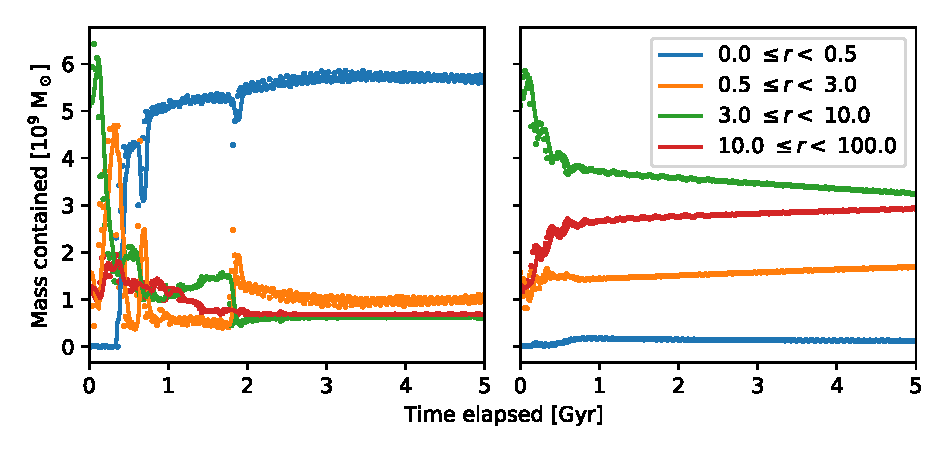
\includegraphics{sd_r_fig.pdf}
    \caption{The evolution of the (gaseous) mass contained within various shells (see legend) is shown. On the left, the {\tt custom} run is show, with the {\tt default} run being shown on the right. It is clear from this figure that the {\tt custom} model causes a large proportion of the gas to be transported into the center of the galaxy; over 80\% of the gas particles falling into this central region within 1 Gyr of the simulation beginning. This is unsurprising as the Toomre $Q$ parameter for the disk in the initial conditions was extremely low (see the discussion in \S \ref{sec:toom_theory} due to the low pressure support that the {\tt custom} model provides.}
    \label{fig:sd_r_evo}
\end{figure}
